%\documentclass[11pt]{article}
\documentclass[article]{IEEEtran}
\usepackage{graphicx}
\usepackage{float}
\usepackage{caption}
\usepackage{amsmath}
\usepackage{amsfonts}
\usepackage[english]{babel}
\usepackage[utf8]{inputenc}
\usepackage[backend=biber]{biblatex}
\usepackage{csquotes}
%\usepackage{docmute}
\usepackage{array}
\usepackage{geometry}
\usepackage[T1]{fontenc}
\addbibresource{plano_de_pesquisa.bib}

\newcommand{\fromeng}[1]{\footnote{do inglês: \textit{#1}}}
\newcommand{\tit}[1]{\textit{#1}}
\newcommand{\tbf}[1]{\textbf{#1}}
\newcommand{\ttt}[1]{\texttt{#1}}

\newcolumntype{C}[1]{>{\centering\let\newline\\\arraybackslash\hspace{0pt}}m{#1}}

\begin{document}

\begin{titlepage}
	\centering
	{\scshape\Large Research Project\par}
	\vspace{1.5cm}
	{\huge \bfseries Attentional models and Deep Learning\par}
	\vspace{1cm}
	{\itshape Erik de Godoy Perillo\par}
	{\itshape Supervisor: Profa. Dra. Esther Luna Colombini\par}
	\vspace{0.5cm}
	\begin{abstract}
        Attention is a fundamental mechanism in intelligent beings.
        It is necessary for filtering the big volumes of stimuli
        constantly arriving and selecting information that is
        important for a certain task.
        Deep Learning is currently broadly applied to Artificial Intelligence.
        The use of attention concepts in current models
        has also been increasingly frequent, resulting many times in
        better results for the task being addressed.
        In this context, this work proposes the elaboration of
        attentional models based on Deep Learning for problems in Artificial
        Ingelligence.
        We aim at obtaining frameworks more generically applicable in broad
        problem classes such as computer vision, Natural Language Processing,
        Differential Computation and others.
	\end{abstract}
	\vfill
	State University of Campinas
	\vfill
	{\large \today\par}
\end{titlepage}

\section{Introduction}
We are constantly receiving high volumes of multimodal stimuli
from both external sources -- such as visual, auditive signals --
 and internal sources -- proprioception, memories et cetera.
It would be very inefficient to proccess all the information with
the same intensity given that a big portion of it is irrelevant for
the task being executed at the moment and we have limited cognitive capacity.
When we read, our vision does not focus on all
words equally, but rather on a small subset of the text at a time.
When we're addressing a given subject, it tends to mediate the focus
in the memory search process, essentially retrieving memories that
are useful for the subject: many other irrelevant memories are not used.
It often happens that something conspicuous
-- such as a bird abruptly appearing in front of us or a sudden sound --
quickly draws our focus, `'stealing'' it from what was previously
being focused on.
The ability to filter and select stimuli that is relevant for a given
cognitive task, keeping the focus for an extended period of time and
directing it to new stimuli when appropriate is fundamental to
human beings and other complex forms of life.
We name this ability `'attention''~\cite{ref:esther-thesis}.

Attention can potentially play an important role in the development
of Artificial Intelligence (AI).
Areas such as computer vision often involve a big quantity of data
and most of time only part of image is relevant to the task at a given moment.
In robotics, attention can be substantially useful:
robots that navigate in complex and dynamic environments need
systems to enable them to handle data from all sensors
so that relevant objects and parts of the scene are promoted to
further processing and decision making -- which needs to be done in real time.
Furthermore, paying attention to abrupt changes in the environment
that may affect the robot's navigation is important for
the robustness, success and safety of the application.
Computational models of attention have been elaborated for years.
A classic example is VOCUS~\cite{ref:vocus}, which was proposed to
simulate the visual attention process in humans.
Many of its mechanisms are based in concepts from psychology.

In recent years, there have been significant improvements in
AI due to the popularization of Deep Learning (DL)~\cite{ref:dl}.
As we will discuss in following sections, the technique consists of
artificial neural networks architectured in a hierarquical manner.
DL showed to be effective in a variety of tasks in
computer vision~\cite{ref:imagenet}\cite{ref:segmentation},
audio processing~\cite{ref:wavenet} and Natural Language
Processing (NLP)~\cite{ref:att-all-you-need} mainly due to its ability
to learn what features to be extracted (rather than relying on hand-crafted
features).
Along with the transposition from classic models to DL
approaches, an increasingly high number of works on the field
have been using concepts related to attention in combination with DL
to achieve better results.
One example is image captioning: the task
consists of giving a natural language description of a given image.
The work in ~\cite{ref:img-captioning} shows that the task benefits from
sequentially focusing on different parts of the image in sequence.
It is achieved by the use of an attentional component in the model.
Other examples include linguistic translation~\cite{ref:translation},
audio recognition~\cite{ref:audio} and neural computation~\cite{ref:ntm}.
More examples will be discussed in-depth in following sections.

\begin{figure}
\begin{center}
	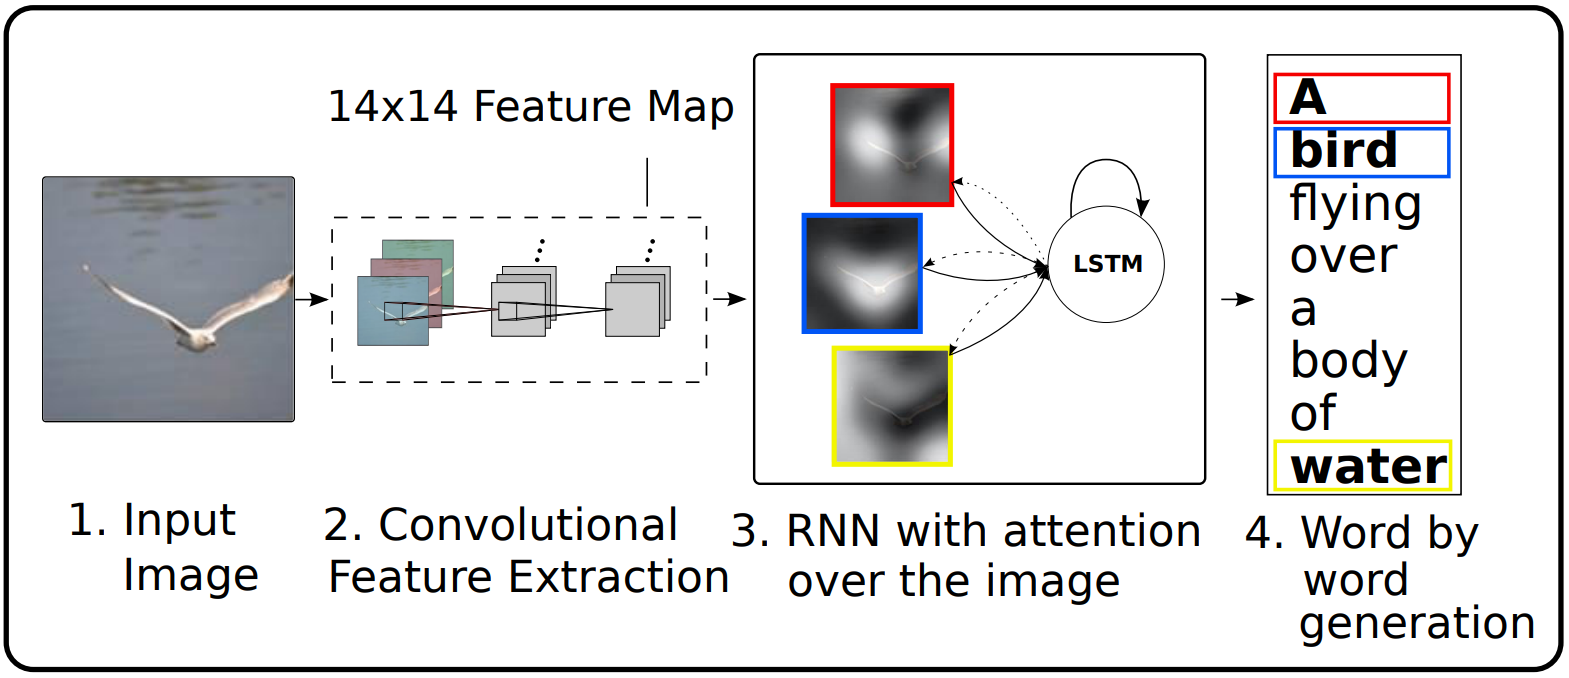
\includegraphics[width=1.0\linewidth]{./img/img_captioning.png}
\caption{
    Diagram of natural language image description using attention
    (from \cite{ref:img-captioning}).
}
\label{fig:description}
\end{center}
\end{figure}

\subsection{Objectives}
The recent adoption of attention by a variety of Deep Learning models 
has shown significant improvements in different tasks.
However, it is conjectured that many other tasks that still don't use
attention would benefit from the concept.
It is believed that a variety of tasks related to robotic navigation,
for example, can be approached by using models with attention.
Furthermore, we note that attention models currently being used
are very specific to each problem in question.
Some works propose a higher level of generalization~\cite{ref:recurr-models},
but we believe it is possible to go further than that.
Therefore, the specific objectives of this work are:
\begin{itemize}
    \item To perform an extensive literature review on the use of attention
        along with modern DL techniques;
    \item To identify specific problems in different classes
        (robotics, vision, NLP, differential programming) with
        improvement potential by the use of attention;
    \item To study the viability of generalization of attention models
        to broader problems in different classes;
    \item To implement the proposed model, evaluating it in an
        application (preferably related to robotics).
\end{itemize}

\section{Background}
\subsection{Deep Learning}
TODO:
\begin{itemize}
    \item brief history and timeline;
    \item hierarquical features
    \item types (cnns, rnns, ntms)
    \item non-convex optimization (SGD etc)
\end{itemize}
\subsection{Attention}
TODO:
\begin{itemize}
    \item definition
    \item general concepts
    \item bottom up
    \item top down
\end{itemize}

\section{Related Work}
TODO: detailed examples on DL + attention.
maybe cite our previous work here?
%In vision, we can cite problems such as visual saliency
%(figure \ref{fig:saliency}): In a given image, which region should be
%first focused on? Older computacional models generally extracted
%hand-crafted features regarding color, luminance and image 
%statistics~\cite{ref:judd}.
%A significant boost in performance~\cite{ref:mit300-bm} was achieved
%with the adoption of Deep Learning models with arquitechture components
%specifically designed for the context of saliency detection ~\cite{ref:deepfix}
%~\cite{ref:salicon}~\cite{ref:mlnet}.
%In previous work~\cite{ref:erik-esther}, which is result from a Undergraduate
%Research project conducted by the author
%-- and received `'best undergraduate research project'' award from
%the institute of computing at Unicamp in 2017 -- 
%we developed a fully convolutional neural network that emcompasses
%arquitechture and data processing specifically design for the saliency
%detection task.
%While having similar performance to that of top models
%(in the MIT Saliency Benchmark) at the time,
%the model was composed of significantly less parameters than other models.

\section{Methodology}
TODO:
\begin{itemize}
    \item description of stages: lit review,
        search for problems, generalization, application
\end{itemize}

\subsection{Schedule}
TODO: the schedule.

\printbibliography

\end{document}
